\chapter{全合成：策略与经典路线}\label{ch:b3:total-synthesis}

抗癌药物紫杉醇最早是从太平洋紫杉的
树皮中分离得到的；剥去树皮会使这种生长缓慢的树死亡，
而其供应远远不能满足患者的需要。化学家以两种办法应对：其一是全合成，
表明该分子可由简单原料构建，但路线过长，不适于生产；其二是以
从欧洲紫杉针叶中提取的一种相关化合物为原料进行半合成，
而针叶是可再生的。
本章讨论此类路线如何评价与设计：产率如何连乘，
汇聚策略为何有利，保护基需付出怎样的代价，应先形成哪些键，
以及用这些工具解读三个具有里程碑意义的合成。

\begin{recall}
本科二年级分册讨论了逆合成分析（目标分子、切断、合成子、
合成等价物、官能团转换）、正交保护基、羟醛反应、
罗宾逊成环、维蒂希反应和亚胺正离子化学；本科一年级分册讨论了
保护基与产率。\Cref{ch:b3:asymmetric-synthesis}、
\cref{ch:b3:pericyclic}
和\cref{ch:b3:homogeneous-catalysis}提供了
现代的关键步骤。
\end{recall}

\begin{omfigure}
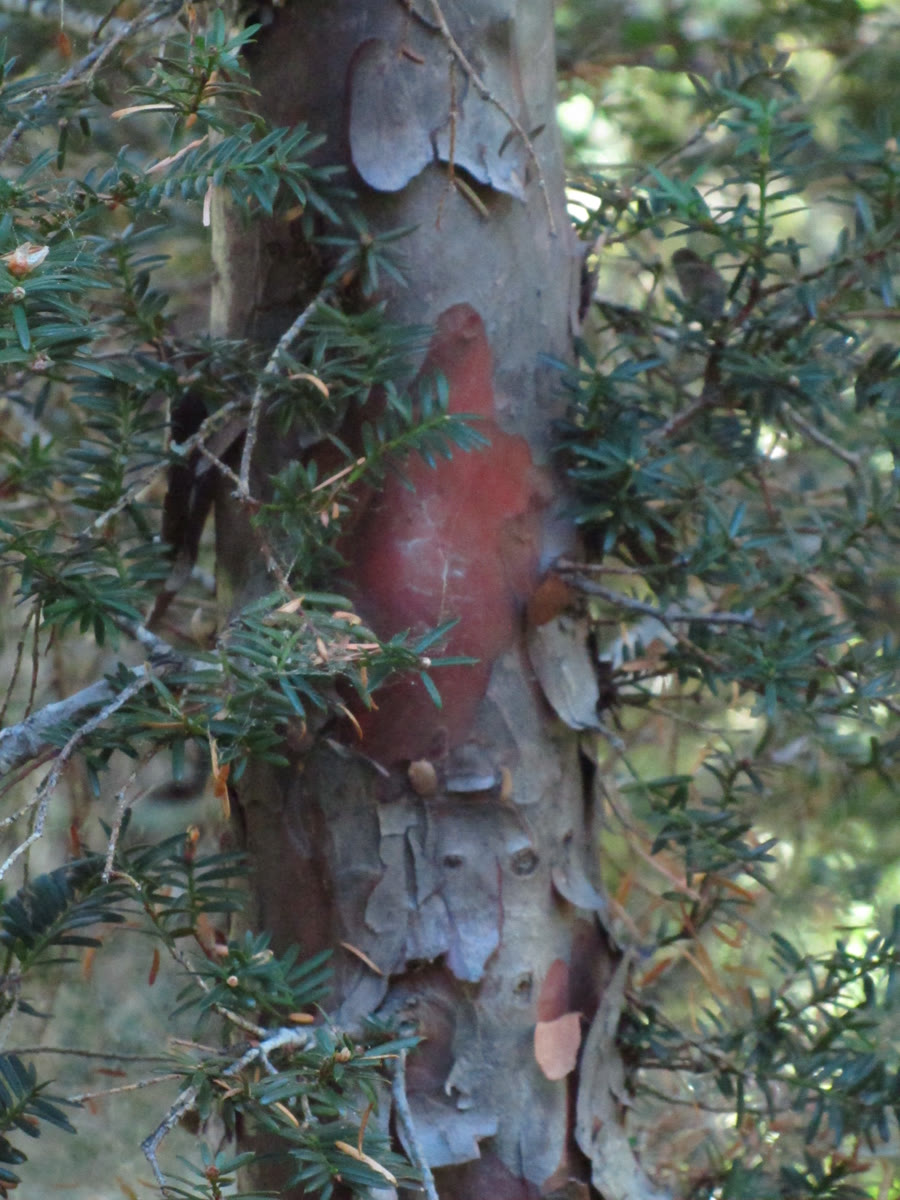
\includegraphics[width=0.32\linewidth]{images/book4/pacific-yew.jpg}

{\small 太平洋紫杉的树皮与针叶，是紫杉醇最初的来源。
摄影：JOE BLOWE, CC BY-SA 2.0.}
\end{omfigure}

\section{合成路线的评价}

\begin{definition}[全合成]\label{def:b3:total-synthesis:total}
由简单的市售化合物制备复杂分子（常为天然产物）的过程称为
\emph{全合成}\index{全合成}。若制得某一全合成路线中的中间体，
则称为\emph{形式合成}\index{形式合成}，即在纸面上完成该路线。
以已接近目标分子的天然化合物为起点的合成称为
\emph{半合成}\index{半合成}。
\end{definition}

\begin{definition}[路线结构]\label{def:b3:total-synthesis:architecture}
在\emph{线性合成}\index{线性合成}中，每一步都作用于前一步的
产物；在\emph{汇聚合成}\index{汇聚合成}中，
各个片段并行制备，并在后期连接。
\emph{最长线性步骤}\index{最长线性步骤}（LLS）是指由任一起始原料
到目标分子所需步骤数的最大值。
\emph{总产率}\index{总产率}是所得目标分子的物质的量
除以限量起始原料的物质的量。
\end{definition}

\begin{proposition}[总产率]\label{prop:b3:total-synthesis:overall-yield}
设一系列步骤的产率依次为 $y_1, \dots, y_n$，则总产率为 $Y = \prod_i y_i$。
\end{proposition}

\begin{proof}
每一步都把所接收的量转化为 $y_i$ 倍的产物，
因此到达目标分子的量，等于起始量依次乘以
每一个因子。
\end{proof}

\begin{proposition}[汇聚]\label{prop:b3:total-synthesis:convergent}
设一条路线共 $n = 2m + 1$ 步，各步产率均为 $y$，由两条各含 $m$ 步的支路
经一步偶联反应连接而成，则其最长线性步骤上的总产率为 $y^{m+1}$，
而同样步数的线性路线的总产率为 $y^{2m+1}$。
\end{proposition}

\begin{proof}
每条支路单独制备，所需起始原料按需供给：每条支路的
物质经过 $m$ 步后再与另一条支路偶联，共 $m + 1$ 个因子 $y$。
在线性路线中，物质须经过全部 $2m + 1$ 步。取 $m = 10$，
$y = 0.90$ 时，两者分别为 31\,\% 与 11\,\%。
\end{proof}

\begin{omfigure}
\begin{tikzpicture}
\begin{axis}[width=0.7\linewidth, height=5.8cm, xmin=0, xmax=30, ymin=0, ymax=1.02,
  axis lines=left, xlabel={步数 $n$}, ylabel={总产率},
  tick label style={font=\scriptsize}, label style={font=\small},
  legend style={font=\scriptsize, draw=none, at={(1.03,0.5)}, anchor=west}, legend cell align=left]
\addplot[color=omDef, thick] table[x=n, y=y95] {figdata/out/bachelor-3-overall-yield.dat};
\addlegendentry{每步 95\,\%}
\addplot[color=omMeth, thick] table[x=n, y=y90] {figdata/out/bachelor-3-overall-yield.dat};
\addlegendentry{90\,\%}
\addplot[color=omThm, thick] table[x=n, y=y80] {figdata/out/bachelor-3-overall-yield.dat};
\addlegendentry{80\,\%}
\addplot[color=omMeth, thick, dashed, mark=*, mark size=1pt] table[x=n, y=y90] {figdata/out/bachelor-3-overall-yield-b.dat};
\addlegendentry{90\,\%，汇聚}
\end{axis}
\end{tikzpicture}

{\small 图示为每步三种产率下总产率随步数的变化（实线：线性路线），
以及每步 90\,\% 时汇聚路线的总产率（两条等长支路在最后一步连接；虚线）。
20 步、每步 90\,\% 时总产率为 12\,\%；若以汇聚方式完成同样的步骤，
总产率约为其三倍。}
\end{omfigure}

\begin{omfigure}
\begin{tikzpicture}[font=\scriptsize, >=Stealth, node distance=0.9cm,
  st/.style={circle, draw, fill=omDef!15, minimum size=4mm, inner sep=0pt}]
  \foreach \i in {0,...,6} { \node[st] (l\i) at (\i*0.9,1.6) {}; }
  \foreach \i in {0,...,5} { \pgfmathtruncatemacro\j{\i+1} \draw[->] (l\i) -- (l\j); }
  \node[anchor=west] at (6.0,1.6) {线性：6 步，LLS 6};
  \foreach \i in {0,...,2} { \node[st] (a\i) at (\i*0.9,0.6) {}; \node[st] (b\i) at (\i*0.9,-0.6) {}; }
  \draw[->] (a0) -- (a1); \draw[->] (a1) -- (a2); \draw[->] (b0) -- (b1); \draw[->] (b1) -- (b2);
  \node[st, fill=omThm!25] (t) at (3.0,0) {};
  \draw[->] (a2) -- (t); \draw[->] (b2) -- (t);
  \node[anchor=west] at (3.4,0) {汇聚：5 步，LLS 3};
\end{tikzpicture}

{\small 路线树状图：每个圆圈代表一种化合物，每个箭头代表一步。线性路线
的全部物质都要经过每一步；汇聚路线则并行制备两个片段并将其偶联，
因而其最长线性步骤更短。}
\end{omfigure}

\begin{definition}[经济性与理想度]\label{def:b3:total-synthesis:economy}
\emph{步骤经济性}\index{步骤经济性}是以尽可能少的步骤达到目标的追求；
\emph{保护基经济性}\index{保护基经济性}则是
尽可能少地使用保护与脱保护步骤。路线的
\emph{理想度}\index{理想度}是路线中
用于构建骨架或进行必要氧化态改变的步骤所占的比例，即
$(\text{构建步骤} + \text{战略性氧化还原步骤})/(\text{总步骤数})$。
\end{definition}

\begin{proposition}[路线的理想度]\label{prop:b3:total-synthesis:ideality}
仅形成骨架键的一锅法路线理想度为 100\,\%；每一次保护、
脱保护、官能团转换或非战略性氧化还原步骤
都会使其降低。
\end{proposition}

\begin{proof}
由定义直接可得：此类步骤使分母增大，
而分子并不增加。
\end{proof}

\section{保护基及其经济性}

每个保护基至少额外占用两步：引入保护基和脱去保护基所需的试剂，
以及两步中损失的物质。一条八步路线若每步产率为 90\,\%，最终保留
43\,\% 的物质；若再加入两次保护与两次脱保护，每步均为 95\,\%，则降至 35\,\%。
保护基应选用正交的，使每一种都可以
在不影响其他保护基的情况下脱去；更好的做法是安排步骤的顺序，
使反应性基团在会产生干扰时并不存在，或尚未暴露，
从而不必使用保护基：无保护基合成是一个目标，而非一种奇巧。

\begin{method}[分析全合成路线]\label{met:b3:total-synthesis:analyse}
\begin{enumerate}
  \item 找出目标分子中的环、手性中心和敏感基团。
  \item 找出关键切断，以及正向实现这些切断的反应
        （即战略键）。
  \item 数出步骤数，找出最长线性步骤，并注意路线是否汇聚。
  \item 说明每个手性中心如何被建立（底物控制、助剂、催化剂、
        手性源）。
  \item 列出保护基和其他非理想步骤，并计算总产率
        及理想度。
\end{enumerate}
\end{method}

\begin{method}[步骤计数]\label{met:b3:total-synthesis:count}
\begin{enumerate}
  \item 一步是指以分离（或至少经过后处理）的
        产物结束的一次操作；未经分离的一锅法序列计为一步。
  \item 总步骤数应计入全部步骤；对于最长线性步骤，
        应沿从市售化合物到目标分子的最长路径计数。
  \item 沿最长线性步骤将各步产率相乘，得到总产率。
\end{enumerate}
\end{method}

\section{战略键与关键成环步骤}

\begin{definition}[战略键]\label{def:b3:total-synthesis:strategic-bond}
目标分子的\emph{战略键}是指这样一根键\index{战略键}：
其切断最能简化目标分子，通常是通过断开一个环系或
一次性消去数个手性中心，并且能够通过可靠的反应生成
该键。
\end{definition}

一次同时形成两根键或数个手性中心的成环反应是最常用的手段：
其中第尔斯–阿尔德反应（形成两根 C--C 键，至多四个
手性中心，具有立体专一性，见\cref{ch:b3:pericyclic}），罗宾逊成环
（在酮上构建六元环）、关环复分解
（见\cref{ch:b3:homogeneous-catalysis}）适用于中环和大环，以及串联反应。

\begin{definition}[串联反应]\label{def:b3:total-synthesis:cascade}
\emph{串联反应}\index{串联反应}是指一系列
这样的转化：每一步为下一步产生所需的官能团，
无需分离中间体，也无需加入新的试剂。
\end{definition}

\begin{definition}[仿生合成]\label{def:b3:total-synthesis:biomimetic}
\emph{仿生合成}\index{仿生合成}是模仿
据信天然产物在生物体内的生成途径。
\end{definition}

角鲨烯氧化物在细胞内环化为羊毛甾醇，四个环与七个手性中心
在一个酶促串联反应中一步形成，启发了
威廉·约翰逊的多烯环化反应：在该反应中，一个阳离子从精心设计的多烯一端出发，
经由类椅式过渡态逐环闭合，
构建甾体中的 \textit{trans} 环稠合结构。

\section{里程碑式路线}

\begin{definition}[曼尼希反应]\label{def:b3:total-synthesis:mannich}
\emph{曼尼希反应}\index{曼尼希反应}是烯醇或烯醇负离子
对亚胺正离子的加成，该亚胺正离子由醛与伯胺或
仲胺原位生成，得到 $\beta$-氨基羰基化合物。
\end{definition}

1917 年，罗伯特·罗宾逊合成了托品酮，它是阿托品和
可卡因的双环母核，他在水中以三种简单组分一锅合成，并设想
植物可能也以同样方式构建它：
$\ce{C4H6O2 + CH3NH2 + C5H6O5 -> C8H13NO + 2CO2 + 2H2O}$（丁二醛、甲胺和
丙酮二羧酸）生成托品酮。

\begin{omfigure}
\begin{tikzpicture}[font=\small, >=Stealth]
  \node[align=center] at (-0.5,0) {$\ce{OHC-CH2CH2-CHO}$\\ $+\ \ce{CH3NH2}$\\ $+\ \ce{HO2C-CH2-CO-CH2-CO2H}$};
  \draw[->, thick] (3.0,0) -- (4.7,0) node[midway, above, font=\scriptsize] {缓冲水} node[midway, below, font=\scriptsize] {$-\ce{2CO2}$, $-\ce{2H2O}$};
  \begin{scope}[xshift=6.1cm, yshift=-0.2cm]
    \coordinate (c1) at (-1,0.3); \coordinate (c2) at (-0.8,-0.5); \coordinate (c3) at (0,-0.9);
    \coordinate (c4) at (0.8,-0.5); \coordinate (c5) at (1,0.3); \coordinate (c6) at (0.45,1.15);
    \coordinate (c7) at (-0.45,1.15); \coordinate (n) at (0,0.45);
    \draw[thick] (c1) -- (c2) -- (c3) -- (c4) -- (c5) -- (c6);
    \draw[thick] (c7) -- (c1);
    \draw[thick] (c6) -- (0.12,1.15); \draw[thick] (-0.12,1.15) -- (c7);
    \draw[thick] (c1) -- (n) -- (c5);
    \draw[thick] (n) -- (0,1.6) node[above, inner sep=1pt] {$\ce{CH3}$};
    \draw[thick, double, double distance=1.5pt] (c3) -- (0,-1.55) node[below, inner sep=1pt] {O};
    \node[fill=white, inner sep=0.5pt] at (n) {N};
    \node[font=\scriptsize, anchor=west] at (1.2,0.3) {托品酮};
  \end{scope}
\end{tikzpicture}

{\small 罗宾逊托品酮合成：两次曼尼希反应，第一次为
分子间反应，第二次成环，将三个组分连接起来；
两个羧基使中央的 $\ce{CH2}$ 基团可烯醇化，随后
以二氧化碳的形式离去。双环产物中，N-甲基桥横跨
七元环。}
\end{omfigure}

\begin{proposition}[一锅法合成托品酮]\label{prop:b3:total-synthesis:tropinone}
一锅法合成托品酮依次经历两步曼尼希反应，
再经两次脱羧。
\end{proposition}

\begin{proof}[证明]
甲胺与丁二醛的一个醛基生成亚胺正离子；
丙酮二羧酸的烯醇加成于其上（第一次曼尼希反应）。生成的仲胺
与第二个醛基缩合，生成环状亚胺正离子，
亚胺正离子随后被另一侧酮的烯醇进攻（第二次曼尼希反应），
从而闭合双环。两个 $\beta$-酮酸基团随后脱去 $\ce{CO2}$，$\beta$-酮酸
在温和加热时即会如此。
\end{proof}

埃利亚斯·科里于 1969 年完成前列腺素 $\mathrm F_{2\alpha}$ 的合成，使逆合成分析明确化。
由第尔斯–阿尔德反应构建的双环[2.2.1]庚烯酮带有
环戊烷取代基的相对构型；
经拜耳–维利格氧化（见\cref{ch:b3:radicals-carbenes}）及
碘内酯化转化为科里内酯，两个侧链由此
经烯化反应连接。该内酯此后已用于
许多前列腺素类药物。

\begin{omfigure}
\begin{tikzpicture}[font=\small,
  box/.style={draw, rounded corners, align=center, fill=omDef!8, inner sep=4pt}]
  \node[box] (t) at (0,0) {前列腺素 \\ $\mathrm F_{2\alpha}$};
  \node[box] (l) at (4.4,0) {科里内酯 \\ （四个 \\ 手性碳原子）};
  \node[box] (b) at (9.2,0) {双环[2.2.1]-\\ 庚烯酮};
  \node[box] (d) at (9.2,-2.4) {取代环戊二烯 $+$\\ 烯酮等价物};
  \draw[omretro] (t) -- (l) node[midway, above=3pt, font=\scriptsize] {烯化反应};
  \draw[omretro] (l) -- (b) node[midway, above=3pt, font=\scriptsize, align=center] {碘内酯化，\\ 拜耳–维利格氧化};
  \draw[omretro] (b) -- (d) node[midway, right, font=\scriptsize] {第尔斯–阿尔德反应};
\end{tikzpicture}

{\small 科里的前列腺素 $\mathrm F_{2\alpha}$ 逆合成路线概要（双箭头表示“由
……制得”）。两个侧链先被切断；
带有四个手性碳原子的环戊烷来自内酯，内酯又来自双环酮，
而酮来自一次第尔斯–阿尔德反应，该反应确定了它们的相对
构型。}
\end{omfigure}

奥司他韦是一种流感药物，工业上由莽草酸制得，莽草酸是一种
手性源化合物，从八角中提取，后来也可通过
发酵制得：其六元环与手性碳原子已预先就位。
该路线先将环二醇转化为环氧化物，用叠氮化物开环，再闭合
成氮丙啶，再以叠氮化物开环，使两个氮原子
\textit{反式}排布；乙酰化与还原完成了合成。由于叠氮化钠与
有机叠氮化物大规模使用时有毒且可能爆炸，此后发展出
无叠氮路线。

\begin{omfigure}
\begin{tikzpicture}[font=\scriptsize, >=Stealth,
  box/.style={draw, rounded corners, align=center, fill=omMeth!8, inner sep=3pt}]
  \node[box] (a) at (0,0) {($-$)-莽草酸 \\ （手性源）};
  \node[box] (b) at (3.1,0) {酯、缩酮、\\ 甲磺酸酯};
  \node[box] (c) at (6.0,0) {环氧化物};
  \node[box] (d) at (8.6,0) {叠氮醇};
  \node[box] (e) at (8.6,-1.5) {氮丙啶};
  \node[box] (f) at (5.4,-1.5) {\textit{反式}-二胺 \\ 前体（叠氮化物）};
  \node[box] (g) at (1.6,-1.5) {磷酸 \\ 奥司他韦};
  \draw[->] (a) -- (b); \draw[->] (b) -- (c); \draw[->] (c) -- (d) node[midway, above] {$\ce{N3-}$};
  \draw[->] (d) -- (e); \draw[->] (e) -- (f) node[midway, above] {$\ce{N3-}$};
  \draw[->] (f) -- (g) node[midway, below, align=center] {乙酰化，\\ 还原};
\end{tikzpicture}

{\small 由莽草酸合成奥司他韦，仅列关键阶段：天然环及其
手性碳原子保留不变，两个氮原子彼此呈 \textit{反式}，
通过依次以叠氮化物开启环氧化物和氮丙啶而引入。}
\end{omfigure}

\section{从发现到工艺}

能提供毫克量样品用于生物测试的路线，很少同时适用于
吨级生产。工艺化学家选择路线时，着眼于成本、安全性与稳健性：
他们以结晶取代色谱法，替换危险的
试剂与低温条件，缩短合成路线，用量热法检验每一步的热安全性，
并为杂质制定规格。
这些选择符合在\cref{ch:b3:green-industrial}中讨论的测量标准。

\begin{inthelab}[从一克到一千克]
在圆底烧瓶中以一克规模进行的一步，在
带夹套的反应器中以十克规模重复，反应器配有顶置搅拌器，并将温度探头
插入液体中，以可控速率加入活性试剂，同时监视
内部温度：放热量随体积增大，而移走热量的
面积只随尺寸的平方增长。只有当热流与后处理
（相分离、过滤、干燥）表现正常时，该步骤才会放大到一千克进行。
\end{inthelab}

\begin{safety}{\ghs[0.62cm]{GHS06}\ghs[0.62cm]{GHS08}\ghs[0.62cm]{GHS09}}
% ledger: ghs4:NaN3
叠氮化钠：吞食致命，对水生生物极具毒性；与酸接触时会
释放出叠氮酸，这是一种有毒且易爆的气体；遇重金属
（排水管中的铜和铅）时会生成易爆的叠氮化物。废液须
经化学方法销毁，绝不可直接倒掉。
\end{safety}

\begin{history}[罗宾逊、伍德沃德、科里]
罗伯特·罗宾逊因其在
生物碱及其他植物产物方面的工作获得 1947 年诺贝尔化学奖；他 1917 年的托品酮合成
至今仍以其经济性被人称道。罗伯特·伍德沃德对奎宁、胆固醇、
叶绿素的合成，以及与阿尔贝特·埃舍诺莫泽共同完成的维生素 $\mathrm B_{12}$ 合成，使全合成成为一门艺术
（1965 年获奖）。埃利亚斯·科里使逆合成分析形式化，并于
1990 年因有机合成的理论与方法获奖。
\end{history}

\section{练习}

\begin{exercise}[$\star$]\label{exo:b3:total-synthesis:1}
计算每步产率分别为 90\,\% 和 80\,\% 时，10 步与 20 步
线性路线的总产率。
\end{exercise}

\begin{exercise}[$\star$]\label{exo:b3:total-synthesis:2}
某路线用五步制得片段 A，用三步制得片段 B，再将两者偶联，
还需再用四步得到目标分子。求出总步数和
最长线性步骤。
\end{exercise}

\begin{exercise}[$\star$]\label{exo:b3:total-synthesis:3}
求丙酮、甲醛与二甲胺发生曼尼希反应
所得的产物。
\end{exercise}

\begin{exercise}[$\star$]\label{exo:b3:total-synthesis:4}
求 4-乙酰基环己烯的第尔斯–阿尔德切断，
并写出正向反应。
\end{exercise}

\begin{exercise}[$\star\star$]\label{exo:b3:total-synthesis:5}
某 21 步线性路线每步产率为 90\,\%。求其总产率及
含两条 10 步支路与一次偶联的汇聚路线的总产率。
\end{exercise}

\begin{exercise}[$\star\star$]\label{exo:b3:total-synthesis:6}
路线 A 共 12 步，其中 7 步构建骨架键，1 步为战略性
还原；路线 B 共 9 步，其中 7 步构建骨架键。求两者的理想度。
\end{exercise}

\begin{exercise}[$\star\star$]\label{exo:b3:total-synthesis:7}
某八步路线每步产率为 90\,\%，需用两个保护基，每个保护基的引入
与脱除产率均为 95\,\%。求使用与不使用保护基时的总产率。
\end{exercise}

\begin{exercise}[$\star\star$]\label{exo:b3:total-synthesis:8}
某三元醇含有伯羟基、仲羟基和叔羟基各一个。提出
能使各羟基依次暴露的保护基，并给出其
脱除条件。
\end{exercise}

\begin{exercise}[$\star\star$]\label{exo:b3:total-synthesis:9}
紫杉醇为何采用半合成法制备，而不是
采用其任何一条全合成路线？
\end{exercise}

\begin{exercise}[$\star\star\star$]\label{exo:b3:total-synthesis:10}
2-甲基环己烷-1,3-二酮与甲基乙烯基酮
发生罗宾逊成环。指出其中的迈克尔加成与羟醛步骤，并给出形成的双环烯酮
（即维兰德–米舍尔酮）。
\end{exercise}

\begin{exercise}[$\star\star\star$]\label{exo:b3:total-synthesis:11}
试证明\cref{prop:b3:total-synthesis:convergent}中的汇聚路线
所需物料比线性路线多 $y^{-m}$ 倍，并计算 $m = 5$ 与
$m = 15$，在每步产率 90\,\% 下计算该因子。
\end{exercise}

\begin{exercise}[$\star\star\star$]\label{exo:b3:total-synthesis:12}
在多烯环化中，为何类椅式过渡态会给出\textit{反式}环稠合，
以及每个双键的几何构型（\textit{E} 或 \textit{Z}）为何重要？
\end{exercise}

\section{问题：一锅法合成托品酮}

\begin{problem}[{周末问题——一锅法合成托品酮：三种组分
及配平方程式、两次曼尼希反应、与长线性路线的比较，
以及托品酮及其还原产物的立体化学}]
\label{pb:b3:total-synthesis:1}
% ledger: aw:C, aw:H, aw:N, aw:O
题目数据：一锅法合成在 pH 约为 5 的缓冲水溶液中进行，
得托品酮，产率为 42\,\%；较早的线性路线需 14 步，每步平均产率为 75\,\%。

\medskip\noindent\textbf{第一部分——组分与方程式。}
\begin{enumerate}
  \item 写出丁二醛、甲胺、丙酮二羧酸
        与托品酮的化学式。
  \item 写出配平的方程式。
  \item 计算反应物及托品酮的摩尔质量。
  \item 计算原子经济性。
  \item 为何用丙酮二羧酸而非丙酮？
  \item 为何在接近中性的 pH 下用缓冲液有利？
\end{enumerate}

\medskip\noindent\textbf{第二部分——反应机理。}
\begin{enumerate}[resume]
  \item 写出第一个亚胺正离子的生成过程。
  \item 写出第一步曼尼希反应。
  \item 第二个亚胺正离子是如何生成的？
  \item 写出第二步的成环曼尼希反应。
  \item 两个羧基为何以 $\ce{CO2}$ 的形式离去？
  \item 数一数所形成的 C--C 键与 C--N 键。
\end{enumerate}

\medskip\noindent\textbf{第三部分——一锅法对比十四步法。}
\begin{enumerate}[resume]
  \item 计算线性路线的总产率。
  \item 计算一锅法产率与之的比值。
  \item 计算一锅法路线的理想度。
  \item 除产率外，还有何因素有利于一锅法路线？
  \item 为何将一锅法合成称为仿生合成？
  \item 列举本章中另一类可一次形成多个键的反应。
\end{enumerate}

\medskip\noindent\textbf{第四部分——立体化学。}
\begin{enumerate}[resume]
  \item 托品酮是否具有手性？找出其对称元素。
  \item 尽管如此，两个桥头碳原子为何仍是手性碳原子？
  \item 酮的还原给出两种醇，即托品醇与假托品醇。其
        二者是什么关系？
  \item 托品醇与假托品醇是否具有手性？
  \item 为何氢负离子优先从羰基的某一面进攻？
  \item 给出结果：一锅法产率与线性路线
        总产率的比值。
\end{enumerate}
\end{problem}
